
%
%Figure \ref{fig:taonta} finally provides a global point of view on layers and
%their relations: $\alpha$ provides abstractions in order to reach meta-levels,
%while $\alpha_1$ and $\alpha_2$ are to be interpreted as projection functions,
%where only data or ontologies are grasped from an enriched context.
%
%As \cite{kleppe} suggests, we need to find a formalism through which express
%data, models and meta-models. We are also interested in defining transforming
%function among those, that is defining different semantic interpretations of
%the same initial concept \cite{saeki}.
%Since we want to make data and model translation possible, we would
%like to express our data relations and structural modification with a modelling language
%that is not necessarily a .
%
%
%By the way the definition of XMI suggests us that it is possible to describe
%the $D$, $M$ and $MM$ layer in the same language representation. Hence
%we want to use a language where we could
%express not only relations between data and models and meta-models, but also
%to express data and model transformations. In order to reach this aim, we have
%to use a system where we could represent data and define queries and transformations
%over it. We would also like to define data transformations over models in the
%same language.

%%%%%%%%%%%%%%%%%%%%%%%%%%%%%%%%%%%%%%%%%%%%%%%%%%%%%%%%%%%%%%%%%%%%%%%%%%%%%%%%%
\subsection{Aggregations}\label{sec:informationsintegration}
\textit{Please observe that this section introduces some running examples that are going to be used along the thesis.}

MOF allows to describe $\alpha$-abstractions between different representation layers but, as previously pointed out, such operator is not allowed to express generalizations inside the same abstraction layer. This consideration implies that other generalization operators working within the same layer (e.g., the \textsc{Data} level) are required. The need of such abstraction mechanism is repeatedly remarked by data modeling literature \cite{Pressman09,Larman04} and in complex systems literature \cite{Johnson2011}, where two distinct types of aggregations are outlined: \textbf{part-of}\index{part of} and \textbf{is-a}\index{is a}\footnote{In \cite{Johnson2011} those two operations are ambiguously called respectively $\alpha$-aggregation and $\beta$-aggregation, or even respectively AND-aggregation and OR-aggregation. Both those notations are not-common in both data modelling and in semantic web literature, where the more explanatory \textbf{part-of} and \textbf{is-a} are used.}. While the \textbf{part-of} relation identifies all the objects that constitute another object within the same abstraction, the \textbf{is-a} relation identifies all the object that could be summarized as one single entity in a coarser representation. Since all those relations are aggregations on the data level, they could be summarized by the following relation, summarizing the information of all the provided objects into one single object \cite{BergamiMM16,BergamiMM17}\index{concatenation!object}:
\begin{equation}\label{eq:nestingAggregation}
\oplus_f\colon\mathcal{P}(D_O)\to D_O
\end{equation}
Please observe that this definition could be used to arbitrarily aggregate a collection of objects through a transformation function $f$. As a consequence, $\oplus$ is part of both the relational \texttt{Join} and  the \texttt{Group By} definition. In the first case, $\oplus$  combines the tuples coming from two distinct relational tables \cite{BergamiMM16}, while in the second it aggregates all the objects belonging to the same equivalence class. Within the relational model, we can suppose that $D_R=\emptyset$: now, we can see that both Join and Group By operators are generalizable using the following \textbf{nesting operator}\index{nesting|see{$\nu$}}\index{$\nu$}:
\begin{equation}\label{def:nestingfirst}
\nu_C^{\oplus_f}(d)=\Set{\oplus_f(\gamma\cap d)|\gamma\in C}
\end{equation}
where $C\in \mathcal{P}(\mathcal{P}(D_O))$ is a collection of collections, and $\nu_C^f\colon \mathcal{P}(D_O)\to \mathcal{P}(D_O)$ transforms a collection of objects into a collection of objects. Given this definition, the join operation within the relational model can be defined as\index{join|see{$\bowtie$}}\index{$\bowtie$!relational}:
\[R\Join_\theta S=\nu^\oplus_{\Set{\Set{a,b|b\in S, \theta(a,b)}|a\in R}}(R\cup S)\]
This means that we select to merge through the tuple combination function $\oplus$ only the tuples that match the predicate $\theta$. Moreover, the Group By can be expressed as follows\index{group by|see{$\gamma$}}\index{$\gamma$!relational}:
\[\gamma^f_{A_1,\dots,A_n}(R)=\nu^f_{\Set{\Set{t'\in R|t[A_1]=t'[A_1],\dots,t[A_n]=t'[A_n]}|t\in R}}(R)\]
This means that we use a generic aggregation function $f$ aggregating the record that share the same common values for the attributes and fields $A_1,\dots,A_n$. Both these operations are used within the relational model for data integration and cleaning purposes \cite{deII}. Consequently, the $\nu_C^{\oplus_f}$ operator can perform both dimensionality reduction and data summarization. 
\begin{figure}[!tp]
	\centering
	\begin{minipage}[!h]{0.7\textwidth}
	\centering
		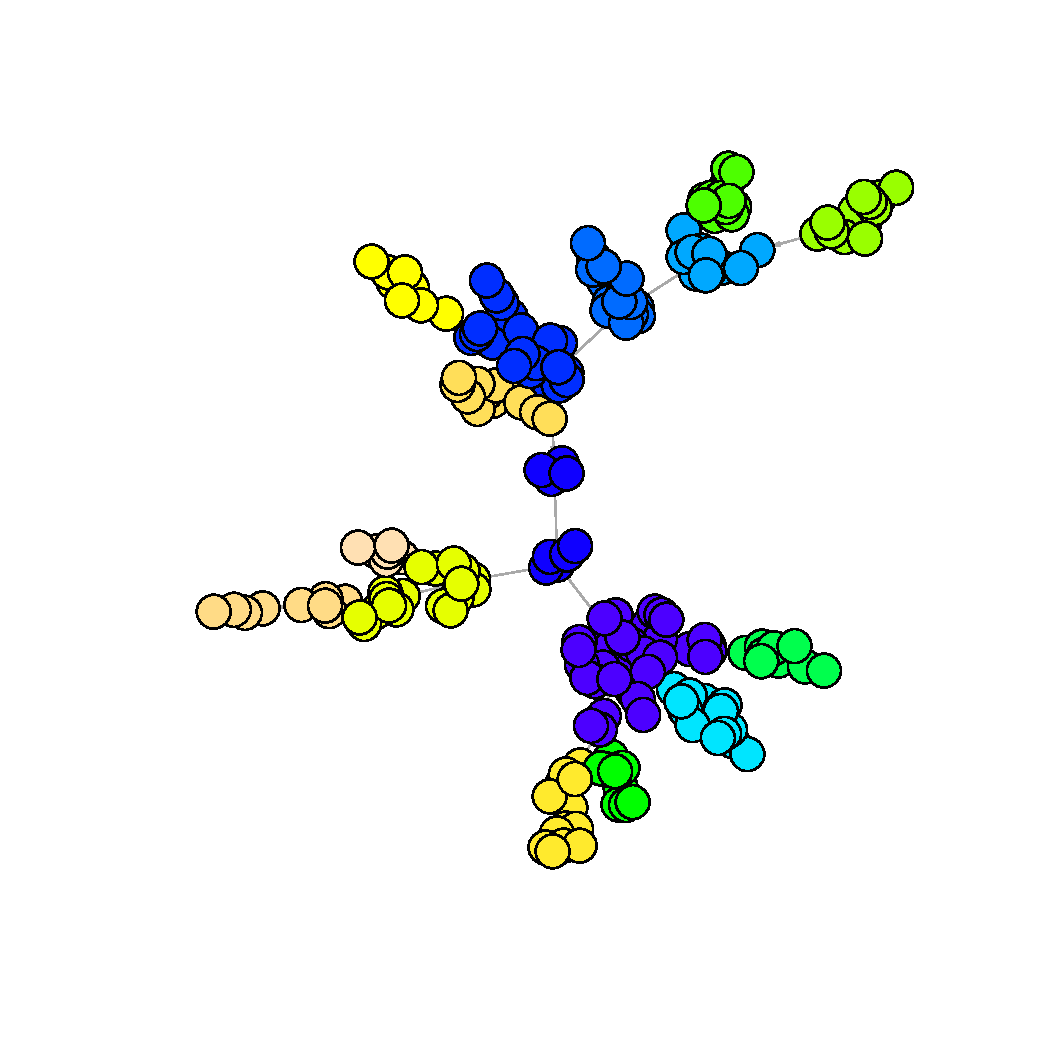
\includegraphics[width=\textwidth]{fig/01dataint/friendgraph}
		\subcaption{An example of an \textit{social network graph} where all the users belonging to the same community are marked with the same colour.}
		\label{fig:communities}
	\end{minipage}
	\begin{minipage}[!h]{0.7\textwidth}
	\centering
		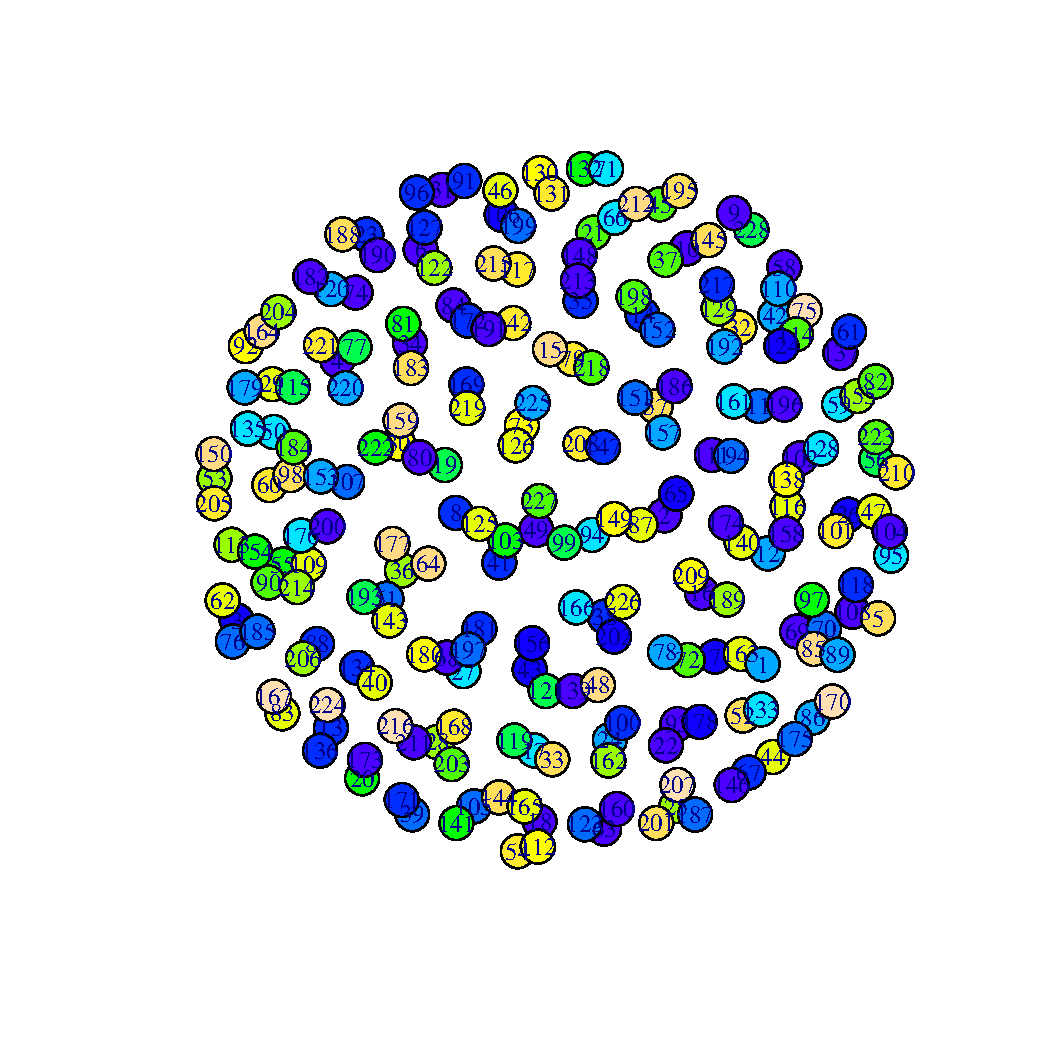
\includegraphics[width=\textwidth]{fig/01dataint/msggraph}
		\subcaption{\textit{Interaction graph} between all the users of the users appearing in the previous graph. Each vertex represents an user and an edge represents that the source user has sent a message to a destination user. We use the same community colours as in the social network graph.}
		\label{fig:interaction}
	\end{minipage}
\caption{Two examples of graph data for social network analysis: a Frienship Graph (\ref{fig:communities}) and an Interaction Graph (\ref{fig:interaction})}
\end{figure}

\begin{figure}[!tp]
	\centering
	\begin{minipage}[!h]{0.7\textwidth}
	\centering
		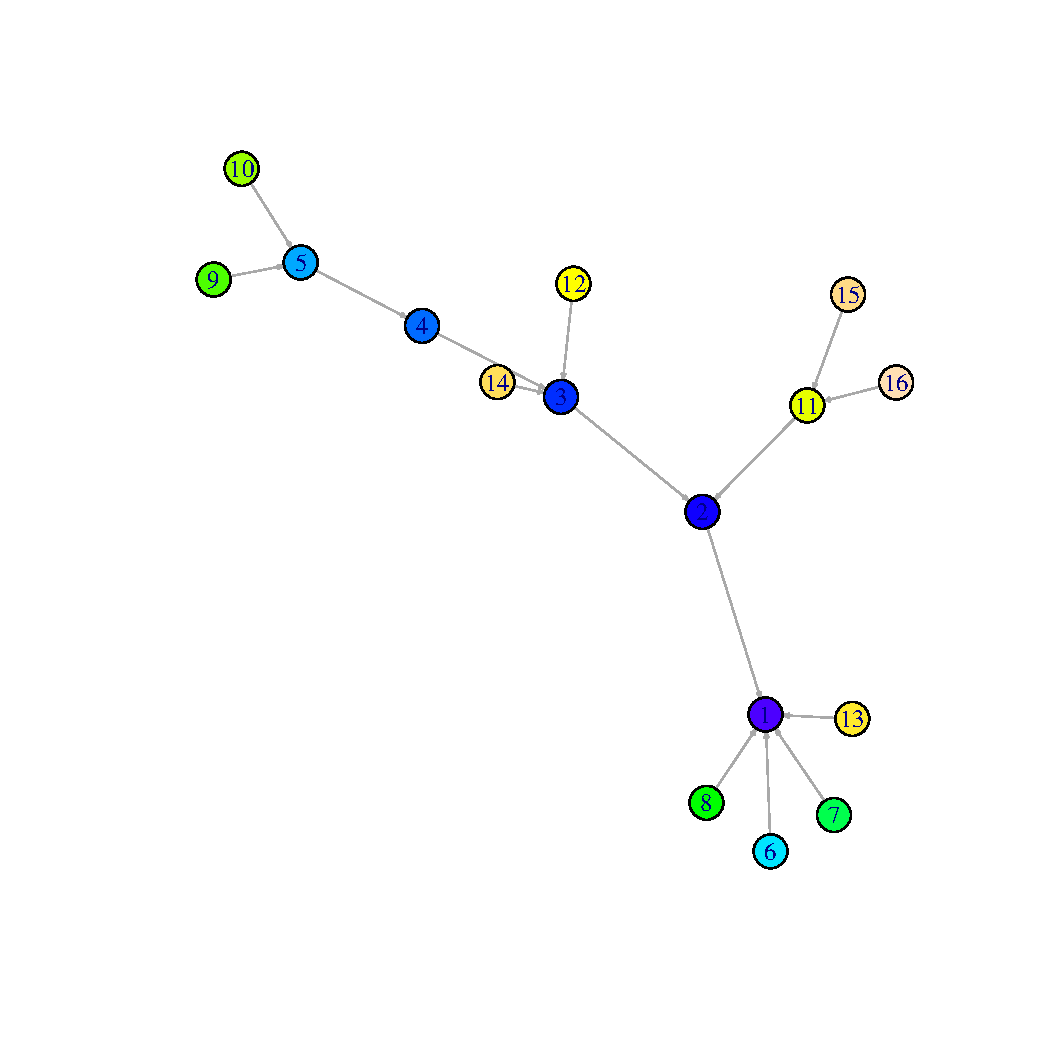
\includegraphics[width=\textwidth]{fig/01dataint/aggregatedSocial}
		\subcaption{Social network graph where all the users belonging to the same community are aggregated together. As a result, there is an edge between one community and another one if one user belonging to the first is friend with another one belonging to the latter.}
		\label{fig:aggrOSN}
	\end{minipage}
	\begin{minipage}[!h]{0.7\textwidth}
	\centering
		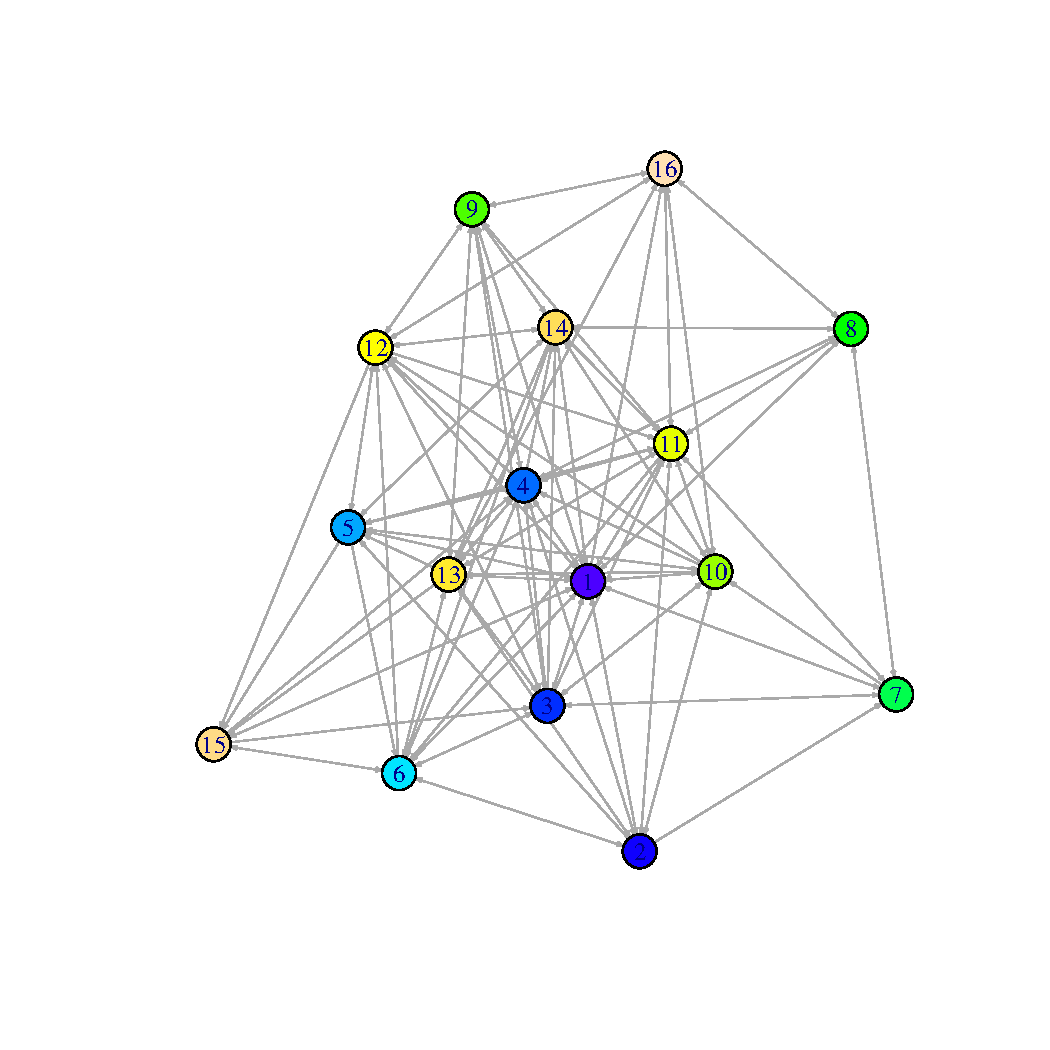
\includegraphics[width=\textwidth]{fig/01dataint/aggregated}
		\subcaption{Upscaling the network interaction at the community level.}
		\label{fig:aggrMSG}
	\end{minipage}
\caption{Coarse grained representation of both the social network graph and the network interaction, aggregated at the community level.}
\end{figure}

\begin{example}\label{ex:8}
The \textbf{part-of}\index{part of|textbf} aggregation could be used within the context of social network analysis, where all the users that belong to an on-line community are \textbf{part-of} such community. Figure \vref{fig:communities} provides an example of a social network graph, where each vertex represents an user and each edge represents a friendship relation. Within the social network scenario, we could be also interested in analyzing the user activities, such as the messages that have been exchanged between the users. An example of such interaction is provided in Figure \ref{fig:interaction}: please note that from this picture is very hard to guess which is the high level perspective of the messages that have been exchanged among the users and which are the kind of interactions among such communities.

Figure \ref{fig:aggrMSG} represents the interaction graph where each user replaced by its corresponding community, thus providing a coarser view of the interaction. At this level, the interaction between the communities is more readable and easier to visualize. Similarly, Figure \ref{fig:aggrOSN} represents a simplified view of the social network graph in Figure \ref{fig:communities}, where the intimacy between social network communities is determined from the friendship relationships between users belonging to different networks.
\end{example}

As we could see from the next example, an operation that only performs an $\nu_C^{\oplus_f}$ aggregation is not enough for establishing new links between the connected components, because as a result of the aggregation result, we could be also interested in establish the relationships between the objects, differently from the former example. Hereby, an operation creating new edges between the objects is required.

\begin{example}\label{ex:bigraphbibnet}
Suppose to have a bipartite graph, where each vertex could be either an author or a paper, and where each edge connects each author to its paper. An example of such graph is provided in Figure \vref{fig:inputbibex}. Moreover, on top of this graph, we want to extract an aggregated\footnote{This problem is addressed in \cite{DMR} and is named \textbf{Graph Projection}. Later on on this thesis (Chapter \ref{cha:nesting}), we're going to show that a graph projection operator shall be defined differently, that is by directly providing an implementation of $\nu_C^{\oplus_f}$.} Co-Authorship graph as the one in Figure \ref{fig:aggrbibex}, where each author internally contains a reference to the papers that he has written. Please observe that the rule establishing the relationships between the resulting vertices here differs from the rule required by the former example: in this example we have to establish an edge between the two aggregated vertex vertices if the original vertices are connected by a path of length $2$, while on the former scenario the path length was $1$. This suggests that another relevant operation in data integration is the establishment of new relationships among the vertices. %This problem will be addressed in Section \ref{subsec:gggSec}, where the Graph Nesting operator will be introduced.
\end{example}

At this point we want to show why the \textbf{is-a}\index{is a|textbf} relation could be represented with a nested representation instead of an \textit{is-a} edge, as currently done in current graph literature. The following example provides an explanation.


\begin{figure}
\centering
\begin{minipage}[!t]{0.6\textwidth}
\centering
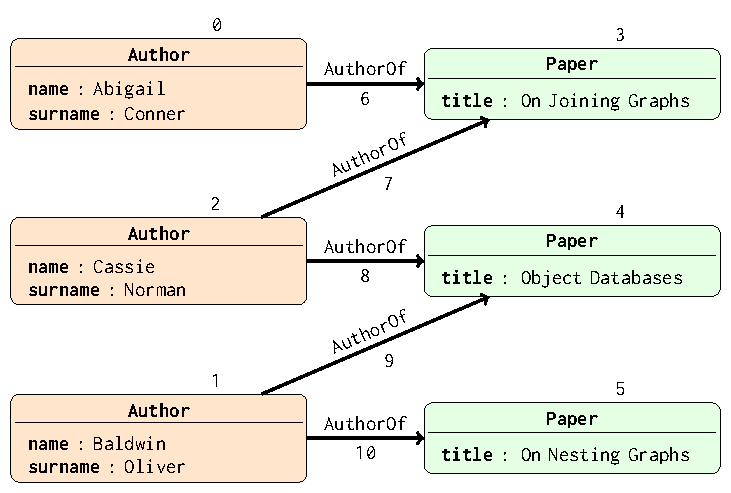
\includegraphics[width=1\textwidth]{fig/01dataint/04bibliography}
\subcaption{Input bibliographical network.}
\label{fig:inputbibex}
\end{minipage} \begin{minipage}[!t]{0.3\textwidth}
\centering
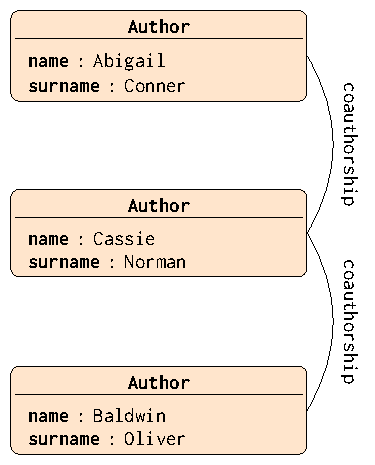
\includegraphics[width=\textwidth]{fig/01dataint/041aggregate}
\subcaption{Aggregated result.}
\label{fig:aggrbibex}
\end{minipage}
\caption{Bibliographic network}
\label{fig:bibex}
\end{figure}


\begin{figure*}[htp]
\centering
\begin{minipage}[t]{0.7\textwidth}
\centering
	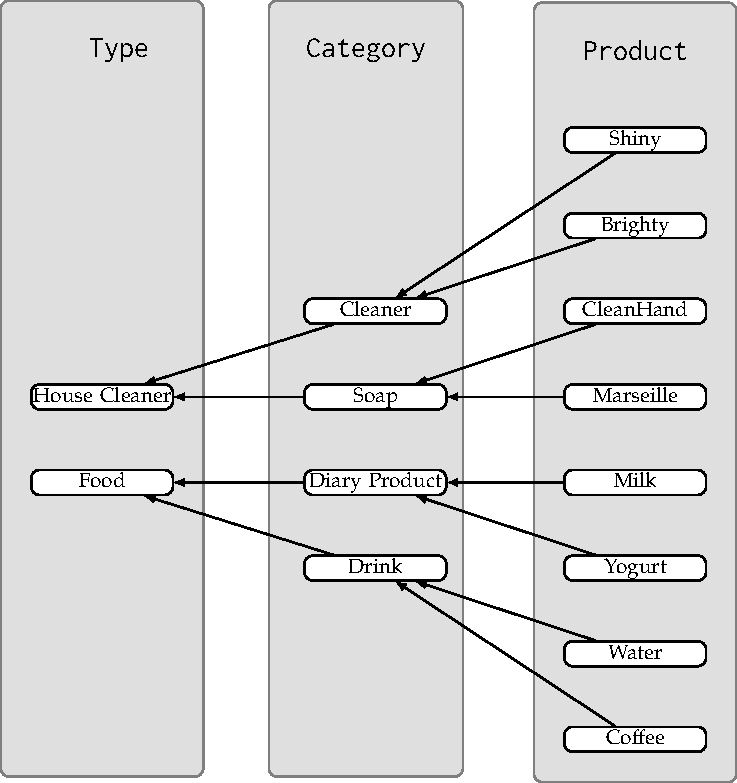
\includegraphics[scale=0.7]{fig/01dataint/00hierarchy}
	\subcaption{Graph and NOF representation, where each edge represent the \textbf{is-a} relation. Each vertex under the same grayed area has the same label of the title of the aforementioned area.}
	\label{fig:hierarchy}
\end{minipage}

\begin{minipage}[t]{0.7\textwidth}
\centering
	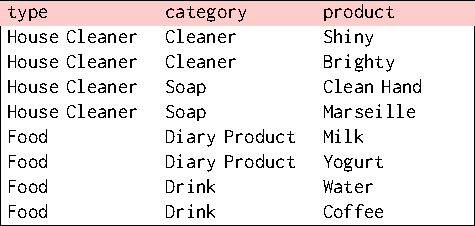
\includegraphics{fig/01dataint/01hiastable}
	\subcaption{Standard relational representation (tabular) within RDBMS for ROLAP data warehouses. Type and category values are replicated for each product.}
	\label{fig:rhierarchy}
\end{minipage}

\begin{minipage}[t]{0.7\textwidth}
\centering
	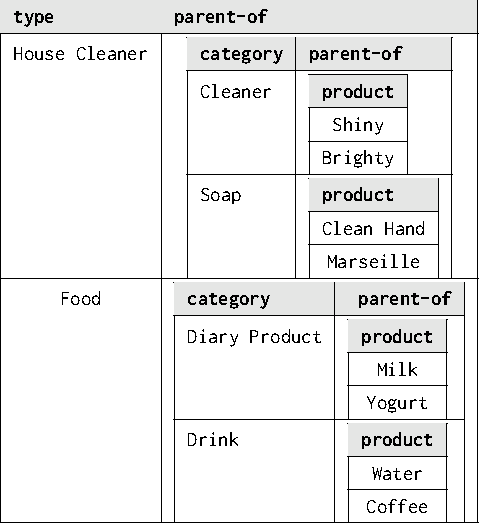
\includegraphics[scale=0.7]{fig/01dataint/02hiasnested}
	\subcaption{Standard nested representation of the \textbf{is-a} hierarchies in Data Warehouses through the inverse relation, \textbf{parent-of}. }
	\label{fig:nhierarchy}
\end{minipage}

\caption{Different representations for a balanced hierarchy describing the taxonomy associated to the products from Figure \vref{fig:umlmodelling}. If we assume that each node represents with a different type, we could completely describe such hierarchy at the model level (see Section \ref{sec:ontology}).}
\end{figure*}

\begin{figure*}[!t]
\centering
\begin{minipage}[t]{0.7\textwidth}
\centering
	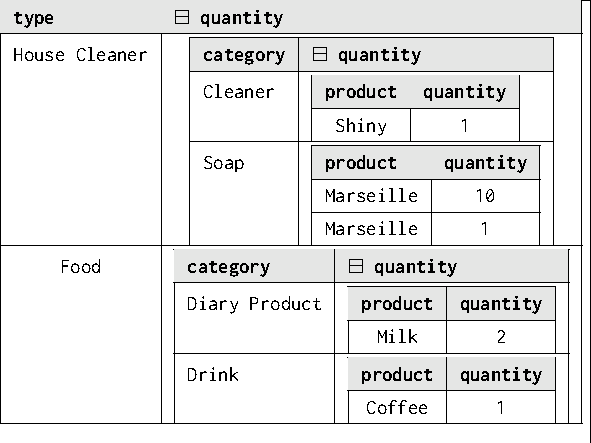
\includegraphics[scale=0.7]{fig/01dataint/030aggregrated}
	\subcaption{Completely expanded components. Each quantity referring to a specific \texttt{SalesOrder} is associated to its product.}
	\label{fig:ag1}
\end{minipage}

\begin{minipage}[t]{0.7\textwidth}
\centering
	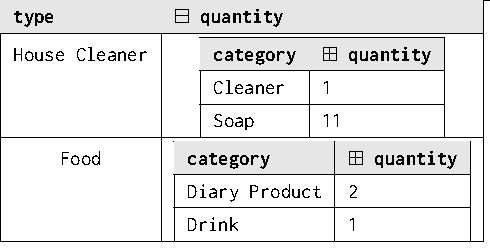
\includegraphics[scale=0.7]{fig/01dataint/031aggregrated}
	\subcaption{Aggregating each product, associating to each category the sum of the sold product within the \texttt{quantity} field.}
	\label{fig:ag2}
\end{minipage}

\begin{minipage}[t]{0.7\textwidth}
\centering
	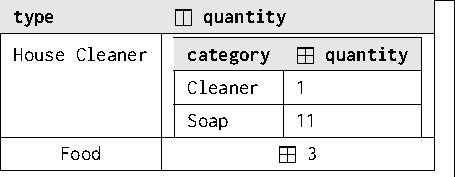
\includegraphics[scale=0.7]{fig/01dataint/033aggregrated}
	\subcaption{Partially expanded components, where only the Food, Cleaner and Soap components are aggregated.}
	\label{fig:ag3}
\end{minipage}

\begin{minipage}[t]{0.7\textwidth}
\centering
	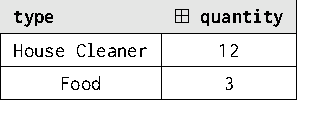
\includegraphics[scale=0.7]{fig/01dataint/032aggregrated}
	\subcaption{Completely aggregated components at the type level. }
	\label{fig:ag4}
\end{minipage}
\caption{Expressing the duality nested relation and aggregated value as provided in modern Data Warehouses \cite{Pentaho,Parra}. $\boxminus$ represents a fully expanded attribute, $\boxplus$ a completely aggregated attribute, and $\boxbar$ a partially aggregated field.}
\label{fig:introducingModel}
\end{figure*}


\begin{example}[label=ex:inaggr]
Suppose to associate a hierarchy to each product within Figure \vref{fig:umlmodelling}, thus allowing to represent vertices at different abstraction levels. Hierarchies are ``\textit{key elements in analytical applications}'' \cite{dwbook} and graphs  allow to provide a direct representation to ``nonstrict hierarchies''. Such graph representation could be also be adopted for transactional data within business process execution \cite{PterMicBergami}, thus allowing to more efficiently represent   the data that has to be joined within a standard relational star schema by simply using edge traversals  \cite{Vasilyeva13,preSQLGraph,SQLGraph}.

Figure \ref{fig:hierarchy} provides an example of a hierarchy for some products in Figure \vref{fig:umlmodelling} at three different abstraction levels. Even though this representation explicitly expresses the \textbf{is-a} relation, it does not provide a good representation of the aggregation. Such aggregation should be represented by the inverse relation of \textbf{is-a}, that is \textbf{parent-of}, and such relation should be an $n$-ary relation containing all its child elements \cite{Johnson2011}; the reason to do this is for associating to each \textbf{parent-of}\index{parent of} relation a value representing the result of the aggregation of the contained elements, that is the result of the $\nu_C^{\oplus_f}$\index{$\nu$} function.

Another standard representation of such hierarchies is provided in Figure \ref{fig:rhierarchy}. In this relational representation  each type and category is replicated for each product. This solution is adopted in order to avoid the navigation cost within relational databases through the join queries. This hierarchy representation, on the other hand, is costly for  hierarchy updates (data updates and removals require a linear scan of the whole table); also, data aggregations are not feasable within this representation and require an additional join and aggregation cost. On the other hand, this hierarchy representation approach is even worse than the former one, because the notion of the \textbf{is-a} relation is completely driven by the ``position of the attributes'' within the table.

The nested relational model, on the other hand, provides a better \textbf{parent-of}\index{parent of} representation by allowing the relations as possible values within a relation's tuple. Figure \ref{fig:nhierarchy} provides an example of how such hierarchy could be modeled within such representation. Even this representation is not beneficial, as within the relational model is not possible to associate to a whole nested relation a data value expressing an aggregated result of its contents.

For this reason, the current thesis will provide in Chapter \ref{cha:graphsdef} a data model where such part-of\index{part of} association is possible, as well as expressing relations between the data as in the graph model. An example of how such dualism (relation and aggregated value) is possible is introduced in Figure \vref{fig:introducingModel}, where we associate to each product the quantity of the goods sold within each \texttt{SalesOrder} (\subref{fig:ag1}). If we consider such aggregation a view over the data, we could think of each aggregated value associated to a nested relation as an expression associated to each of its subcomponents\footnote{\url{http://github.com/jackbergus/-facerei}}. As a consequence, our desired data model should provide both atomic values and expressions composing values and attributes; each \texttt{quantity} field at both the \texttt{type} and \texttt{category} level should provide both the expression $\texttt{sum}(x\mapsto x.\texttt{quantity})$ for the aggregated representation, and a relation over which perform the aforementioned aggregation. Please note that this association could not be provided by the standard nested relational model but, on the other hand, it is frequently used in Data Warehouses for exploring via expansions and collapses the multidimensional components. An example of how o perform such queries is going to be provided later on in Section \vref{subsec:representingisa} through the help of some algebraic operators. Moreover, each component could be arbitrarily expanded or aggregated (\subref{fig:ag3}): therefore such representation could not fit in the nested relational model. This example will extended and discussed within the nested graph model at page \pageref{ex:firstforgrammars}, after providing a query  \textsc{Language} allowing to combine (nested) graph data alongside with other represented within the same general data model.
\end{example}
